% LTeX: language=en-GB
% !TEX root = ../../report.tex
\section{Step 1 - Axial compression test (experimental)}\label{section:step1-test}
\subsection{Implementation}
The pharmaceutical product selected for the characterisation of medical payloads for UAV-based transportation is one of the most fragile phial types currently available on the pharmaceutical market. This choice was deliberate: by characterising a worst-case, low-strength test article, the resulting airbag design is expected to provide adequate protection also for more robust payload cases. The test consisted of a simple compression test, through which the maximum compressive load sustainable by the phial was measured.

Therefore, the parameter of interest for this test was the compressive force at which the phial broke, hereafter referred to as the \textbf{\textit{failure load}} $F_{fail}$, expressed in Newtons. This was the only quantity of interest measured during the test. The failure load constitutes the experimental datum that is used to calibrate the finite element model (FEM) of the compression test in the design workflow's Step 2.


\subsubsection{Test Article}
The test articles were glass phials containing 5\,ml of saline solution, 70\,mm in height, 15\,mm in diameter, with an assumed wall thickness of 0.4 to 0.5\,mm (see \cref{fig:glass-phial}) as shown in \cref{fig:glass-phial}. The saline solution phials represented safe alternatives to phials containing medicinal products of the type used in the typical failure scenario described in \cref{sec:reference-mission}, \cref{fig:akineton}. The choice deliberately addressed safety concerns related to the toxicity of \textit{Akineton Fiale}, to which the testing operators would have been exposed when the tested phials reached their breaking point (see paragraphs on \textit{Test arrangement} and \textit{Test procedure} for clarification, and \cref{sec:safety-analysis} for information on safety precautions). The assumption at the basis of this test procedure was that \textit{the material of which the test articles were made corresponded to the material of the medicinal glass phials} relevant for the reference mission described in \cref{sec:reference-mission}. This assumption was supported by previous investigations of pharmaceutical manufacturers in the Italian and European pharmaceutical landscape \hl{cite pharmaceutical producers here?}. For the purposes of this test, only the mechanical properties of the glass container were of interest.

\begin{figure}[h]
    \centering
    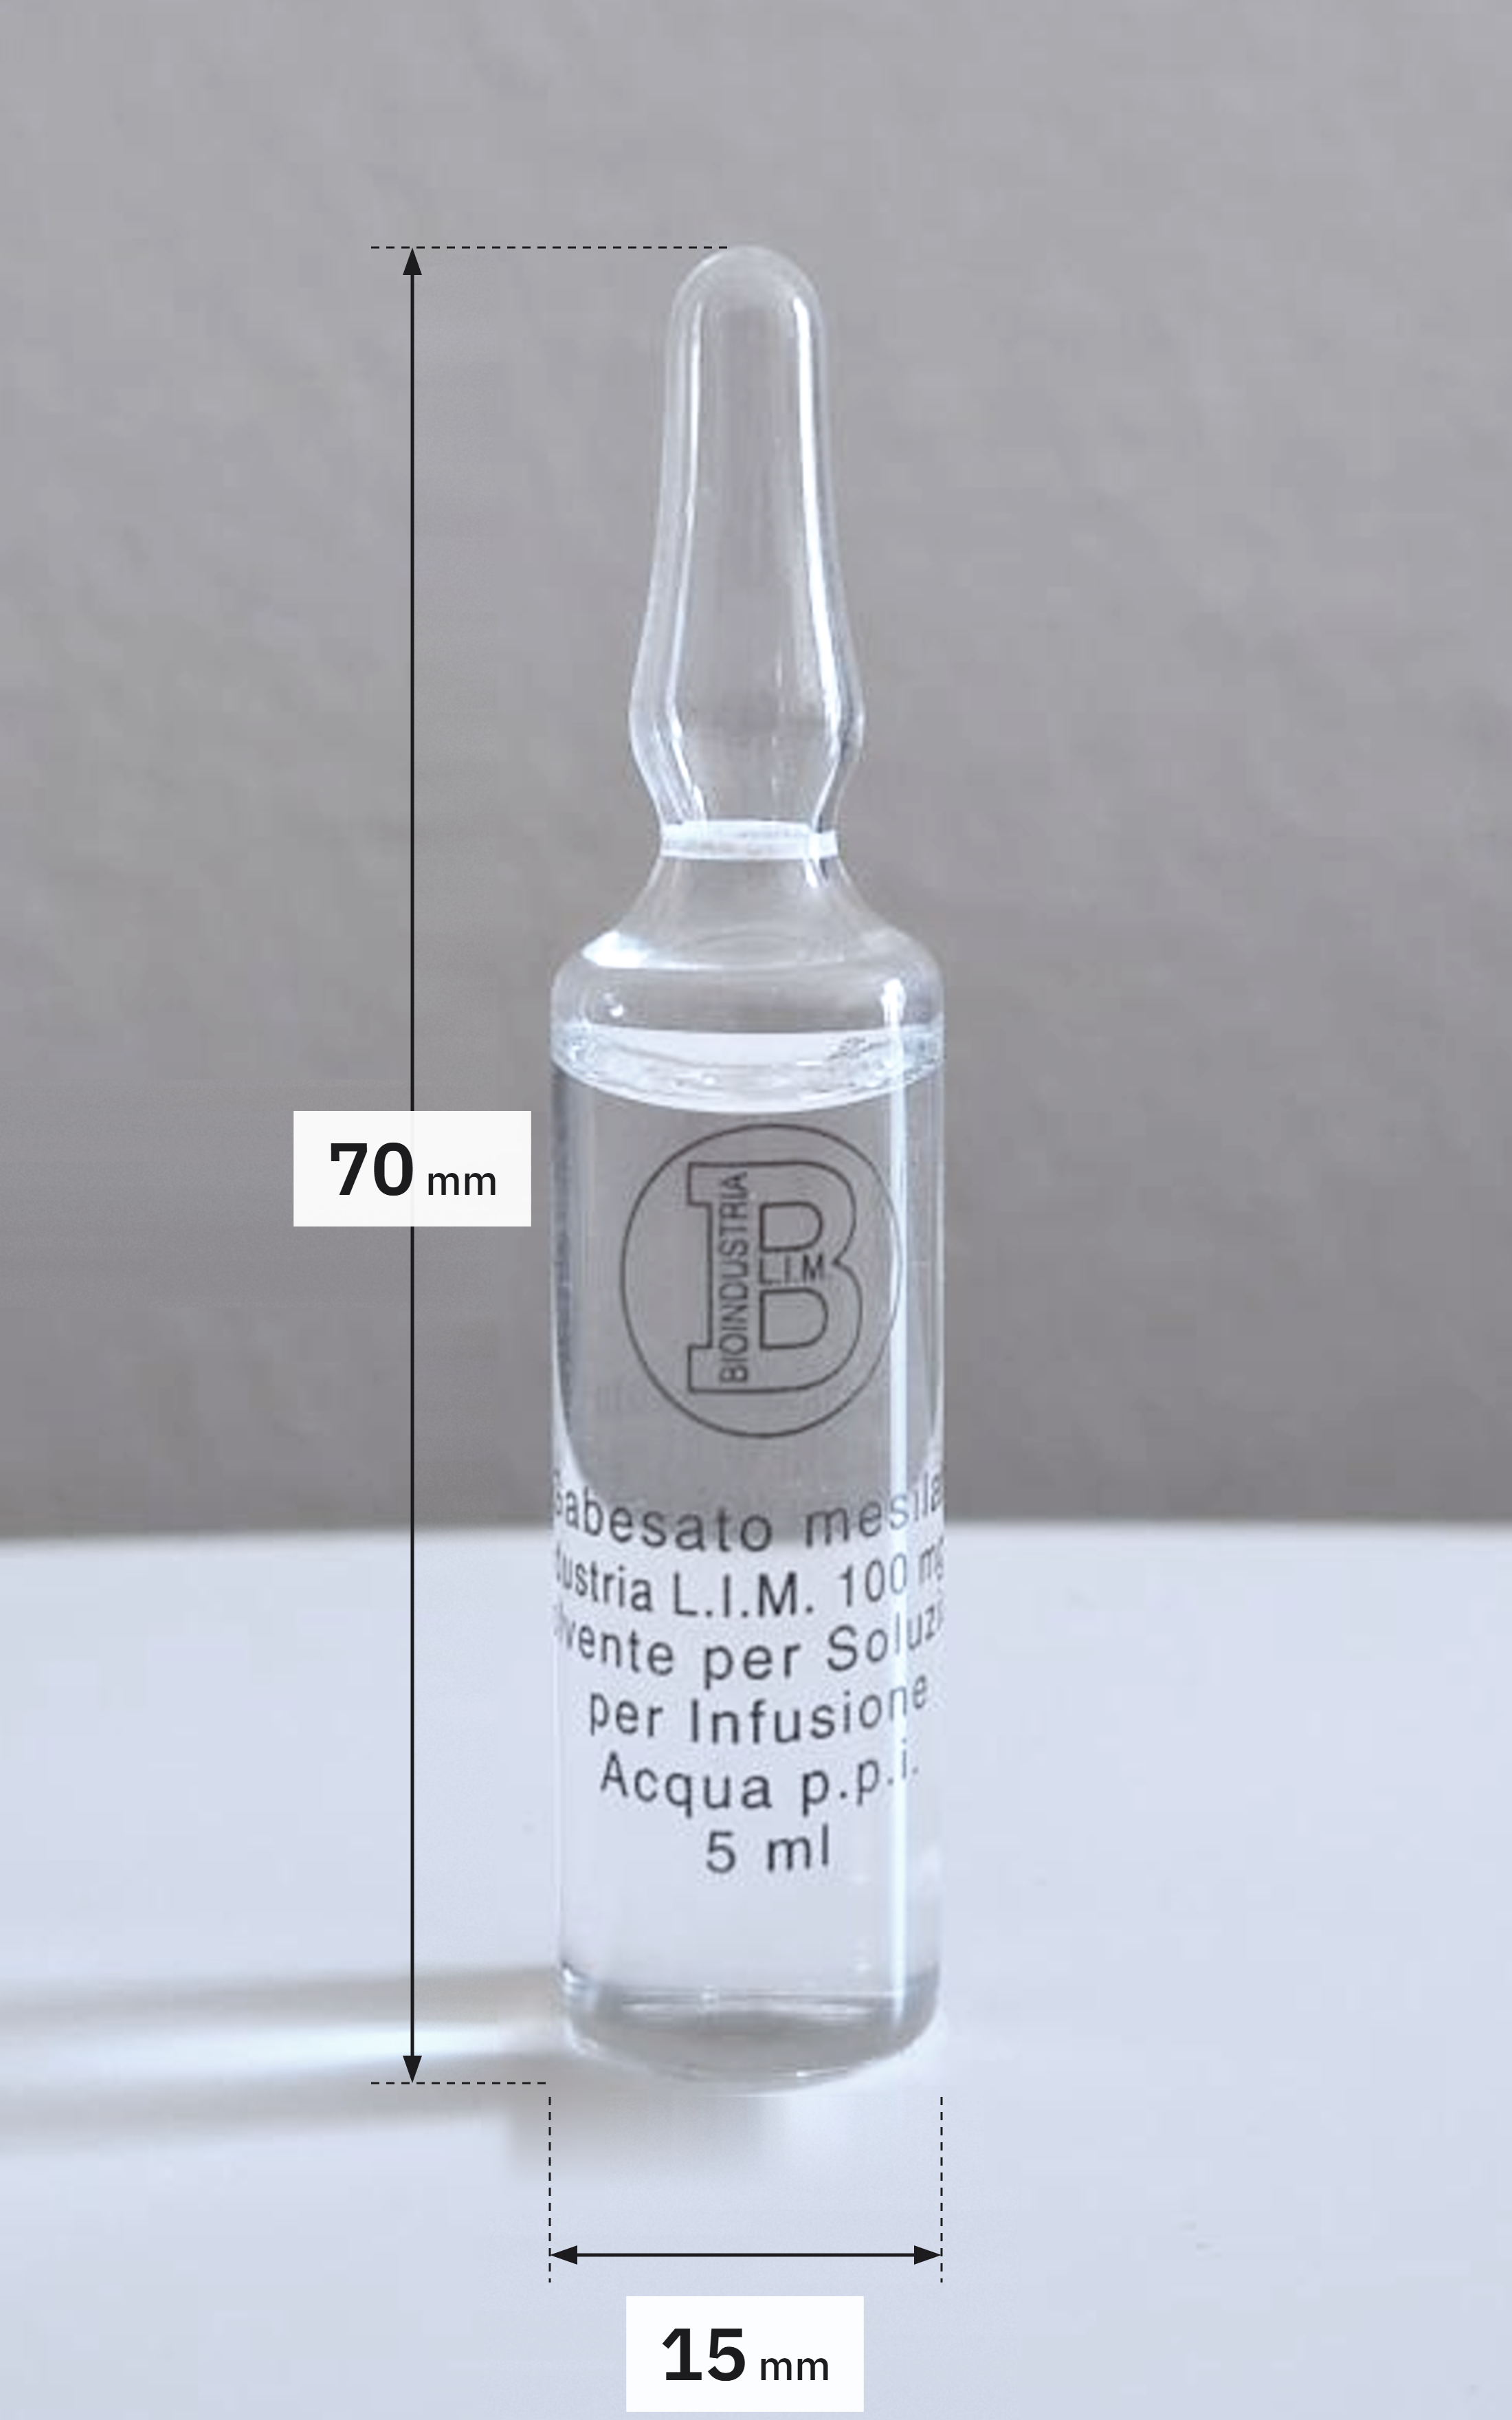
\includegraphics[height=6cm]{figures/chap4/step1-exp/5ml_phial_final.png}
    \caption{Glass phial containing saline solution, annotated with dimensions.}
    \label{fig:glass-phial}
\end{figure}

For the purpose of efficient data analysis, it is important to note that the phials originated from two distinct medicinal batches, designated as Batch A (36 phials) and Batch B (40 phials), provided by different pharmaceutical producers. The initial assumption that all phials share identical geometry and material properties stems from their classification as standardised containers designed to hold 5\,ml of solution. Within the pharmaceutical supply chain, glass container manufacturers typically produce and dispatch these standardised phials to pharmaceutical producers, who subsequently fill them with medicinal product and seal them through specific heat treatments. This implies that parameters such as exact wall thickness variation and specific thermal treatment histories cannot be directly measured prior to testing, and the assumption of the standardised geometric and material properties is ultimately proven incorrect by the experimental results presented in \cref{sec:step1-results}.


\subsubsection{Test arrangement and procedure}\label{sec:test-arrangement}
The compression test was performed using an \textit{MTS QTest/10} testing machine, equipped with a 10\,kN load cell for force measurement and control software \textit{TestWork}. The test setup is shown in \cref{fig:compression_setup}. The phial was held vertically by means of a custom 3D-printed PETG adaptor, which was clamped at its base by the machine's lower clamp. The compression head of the machine, mounted on the moving crosshead, was lowered from above until contact was established with the tip of the phial, after which the compressive load was applied along the phial's longitudinal axis.

\begin{figure}[h]
    \centering
    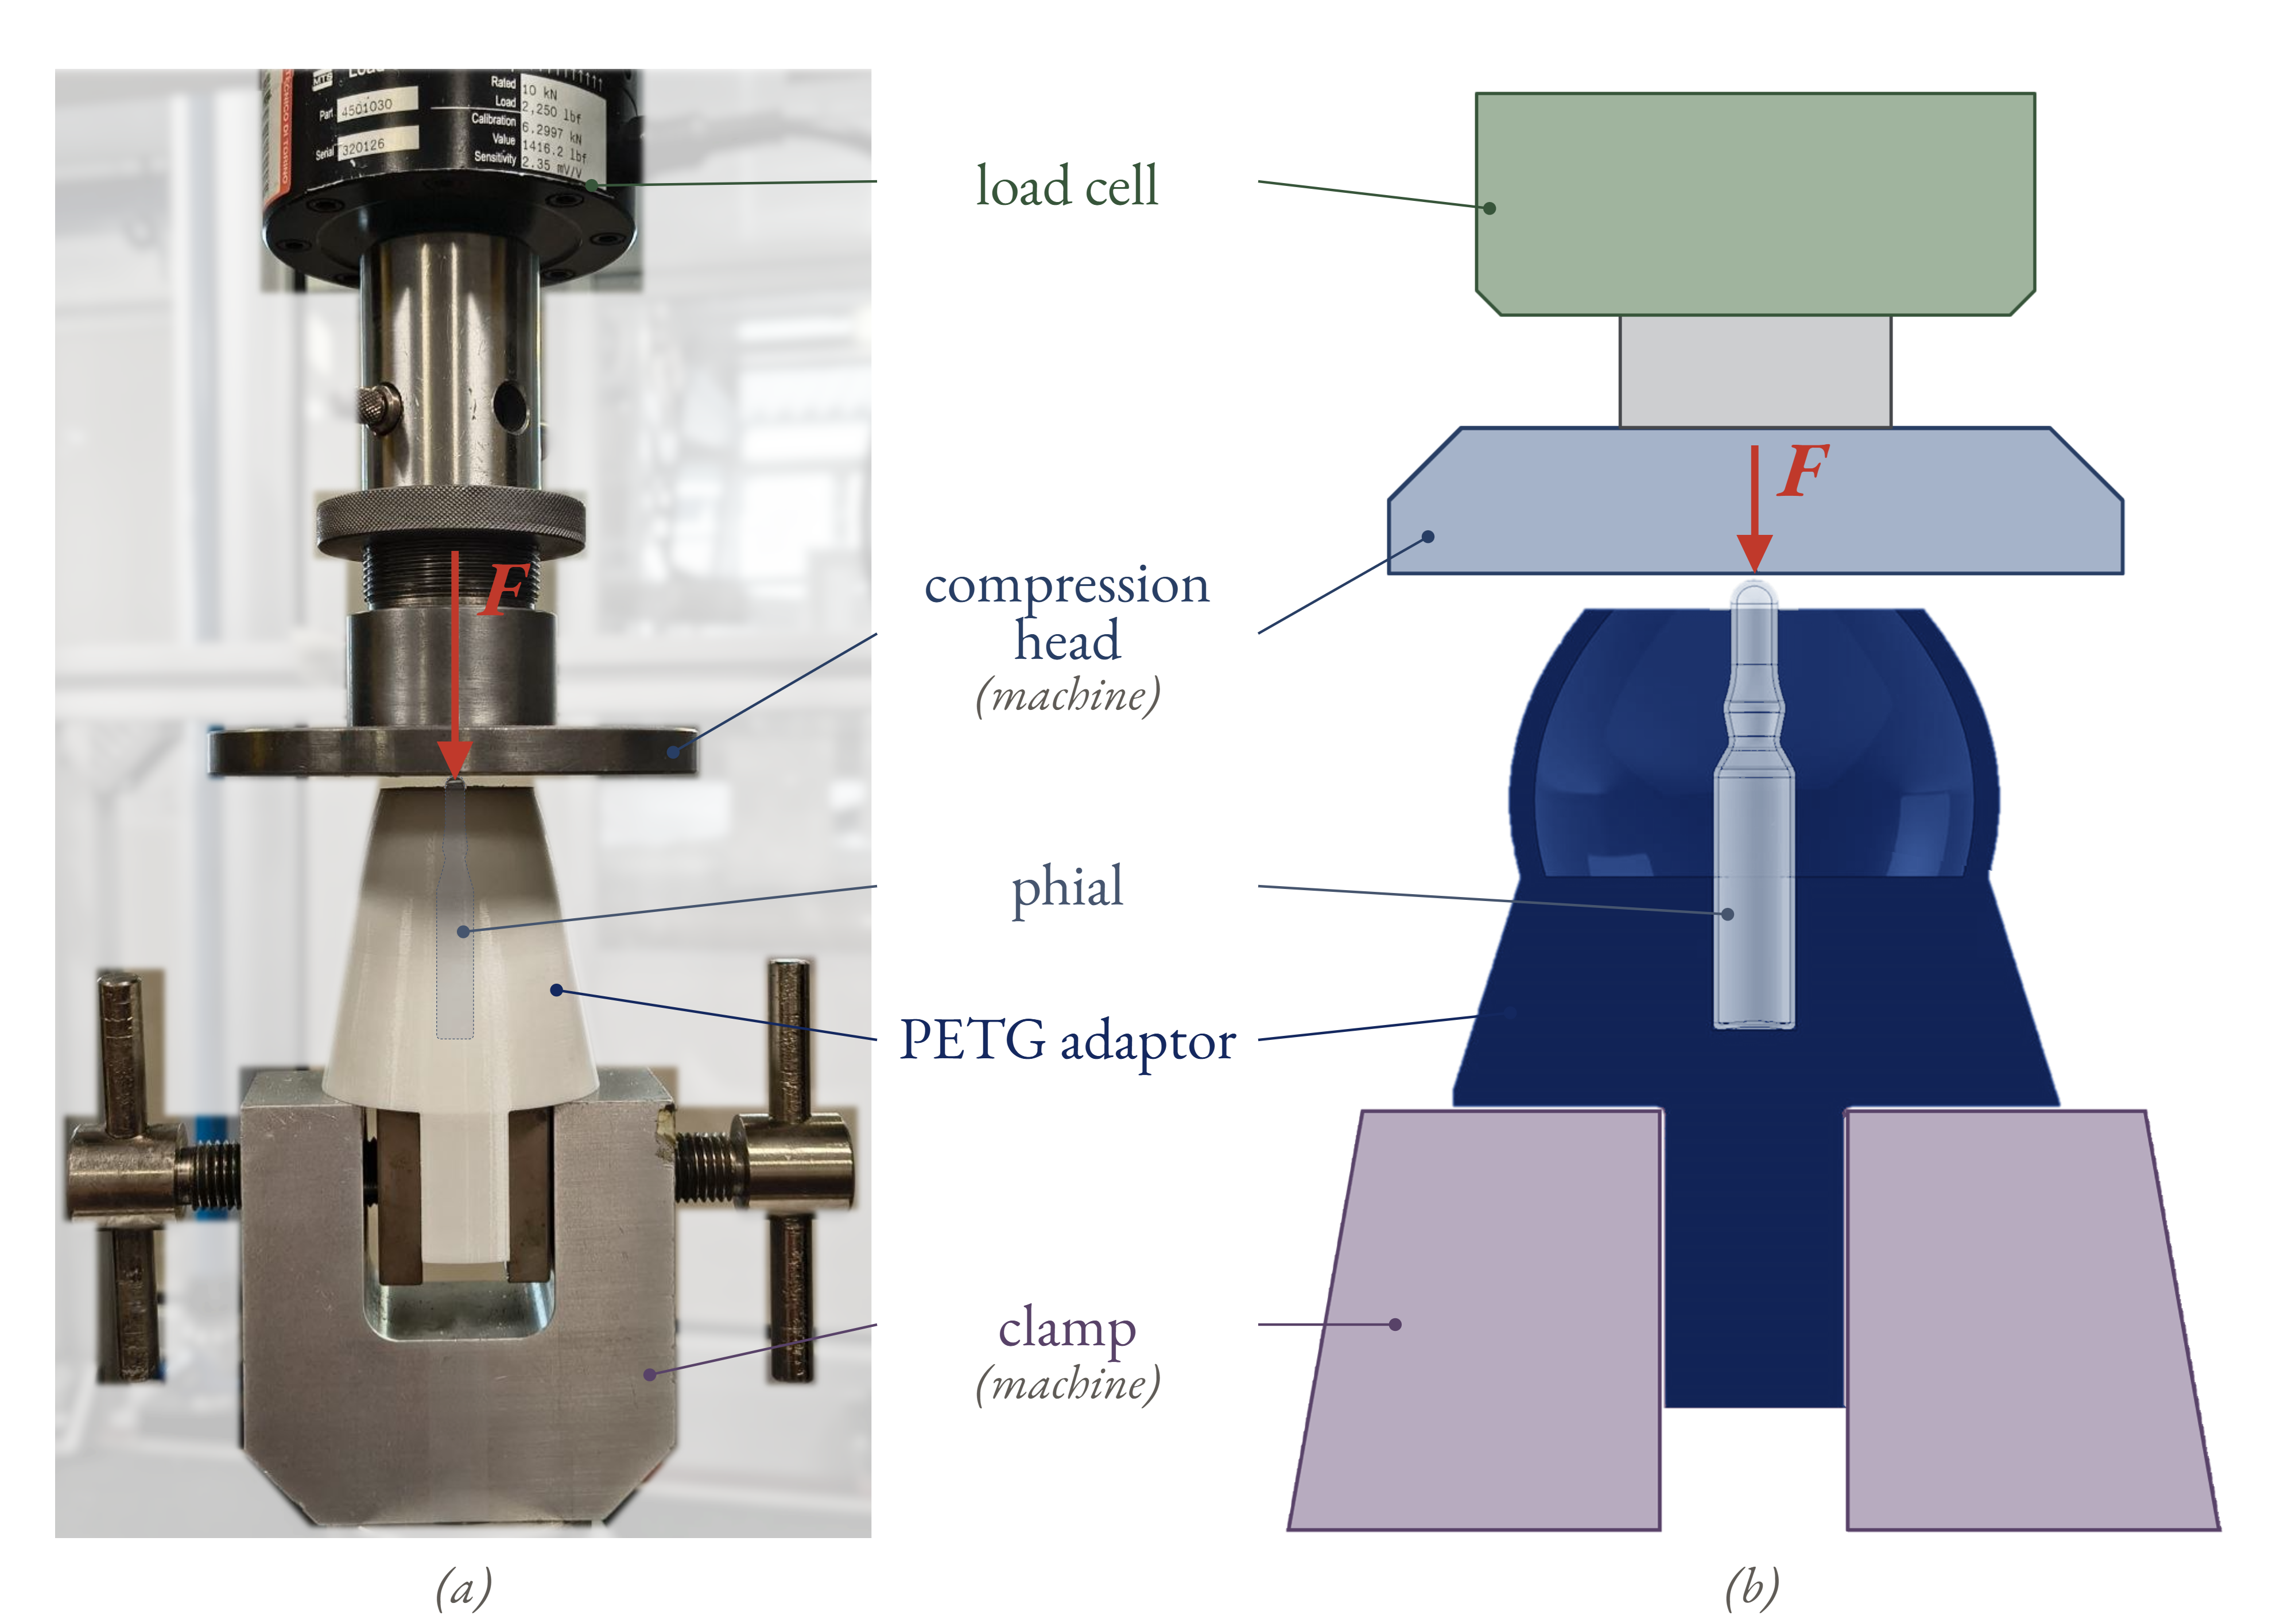
\includegraphics[width=0.8\textwidth]{figures/chap4/step1-exp/exp_setup_final.png}
    \caption{Test arrangement: phial held by a PETG adaptor and lower clamp, with the compression head applying the load from above.}
    \label{fig:compression_setup}
\end{figure}

The machine was operated under velocity control, measured in mm/min. During the test, the applied force was continuously monitored as a function of crosshead displacement, until phial breakage occurred. Breakage was detected by the testing machine as a sudden drop in the measured load, which triggered an immediate, automatic stop of the crosshead motion.


\subsubsection{Test procedure}\label{sec:test-procedure}
The failure load was measured at three displacement rates: 1, 2, and 3 mm/min, which guaranteed the quasi-static nature of the test as the measured failure load was observed to be independent of the applied displacement rate (the variation in failure load across the tested rates fell within the expected scatter of the material).

The compression test was repeated on a batch of 76 nominally identical phials (although belonging to two different medicinal batches) to obtain a statistically meaningful population of failure load values. Each phial was visually inspected for pre-existing damage (e.g., cracks or chips) that could affect the test results and was discarded if any defect was found. The phial was then inserted into the PETG adaptor (cleaned from previous phial tests), ensuring correct vertical alignment and full seating within the adaptor up to the height of the phial's main body. Next, the PETG adaptor, with the phial inserted, was positioned within the lower clamp of the testing machine and secured. The compression head was lowered until contact was established with the tip of the phial, taking care not to apply any preload. Finally, the displacement rate was selected, and the test was monitored until phial breakage occurred (triggering an automatic stop of the crosshead). Displacement and applied load data were continuously recorded for each phial.



\subsection{Results}\label{sec:step1-results}
The medicinal phials under study are not designed as standard coupons to test material properties. In addition, it is important to consider a second complication related to the material of \textit{glass} itself, notoriously characterised by great scatter in mechanical properties. For these two reasons, it is key to introduce some statistical analysis in analysing the experimental results, specifically adopting a two-parameter Weibull distribution parameters to study the phials behaviour. The Weibull distribution is widely recognised in the literature as the most appropriate statistical model for describing the strength of brittle materials like glass due to its ability to capture the weakest-link nature of brittle fracture, which is governed by the size and distribution of surface flaws \cite{datsiou2018weibull}. Several of the observations were made empirically, i.e. just by looking at the breaking modes or even listening to sound cues in the laboratory, as the almost artisanal setup comes with strong limitations.


\subsubsection{Phial breaking modes and statistical observations}
Prior to conducting the experimental campaign on the glass phials, it was hypothesised that the phials would break in five areas of potential stress concentration along their geometry. \Cref{fig:breaking-modes} illustrates these critical areas: the phial's dome \textit{A}, the first bulge \textit{B}, the necking \textit{C} (the failure point designed to open the phial), the base \textit{D}, and the main body wall \textit{E}. During the tests, it was noticed that not all breaking modes would manifest and that a significant portion of the broken samples would show a combination of two or three failure modes, described as \textit{hybrid} failure modes from this point onwards. \Cref{fig:breaking-modes} is a qualitative diagram of various failure modes and exemplifies their nature through pictures taken throughout the testing campaign to accompany empirical observations.

\begin{figure}[h!]
    \centering
    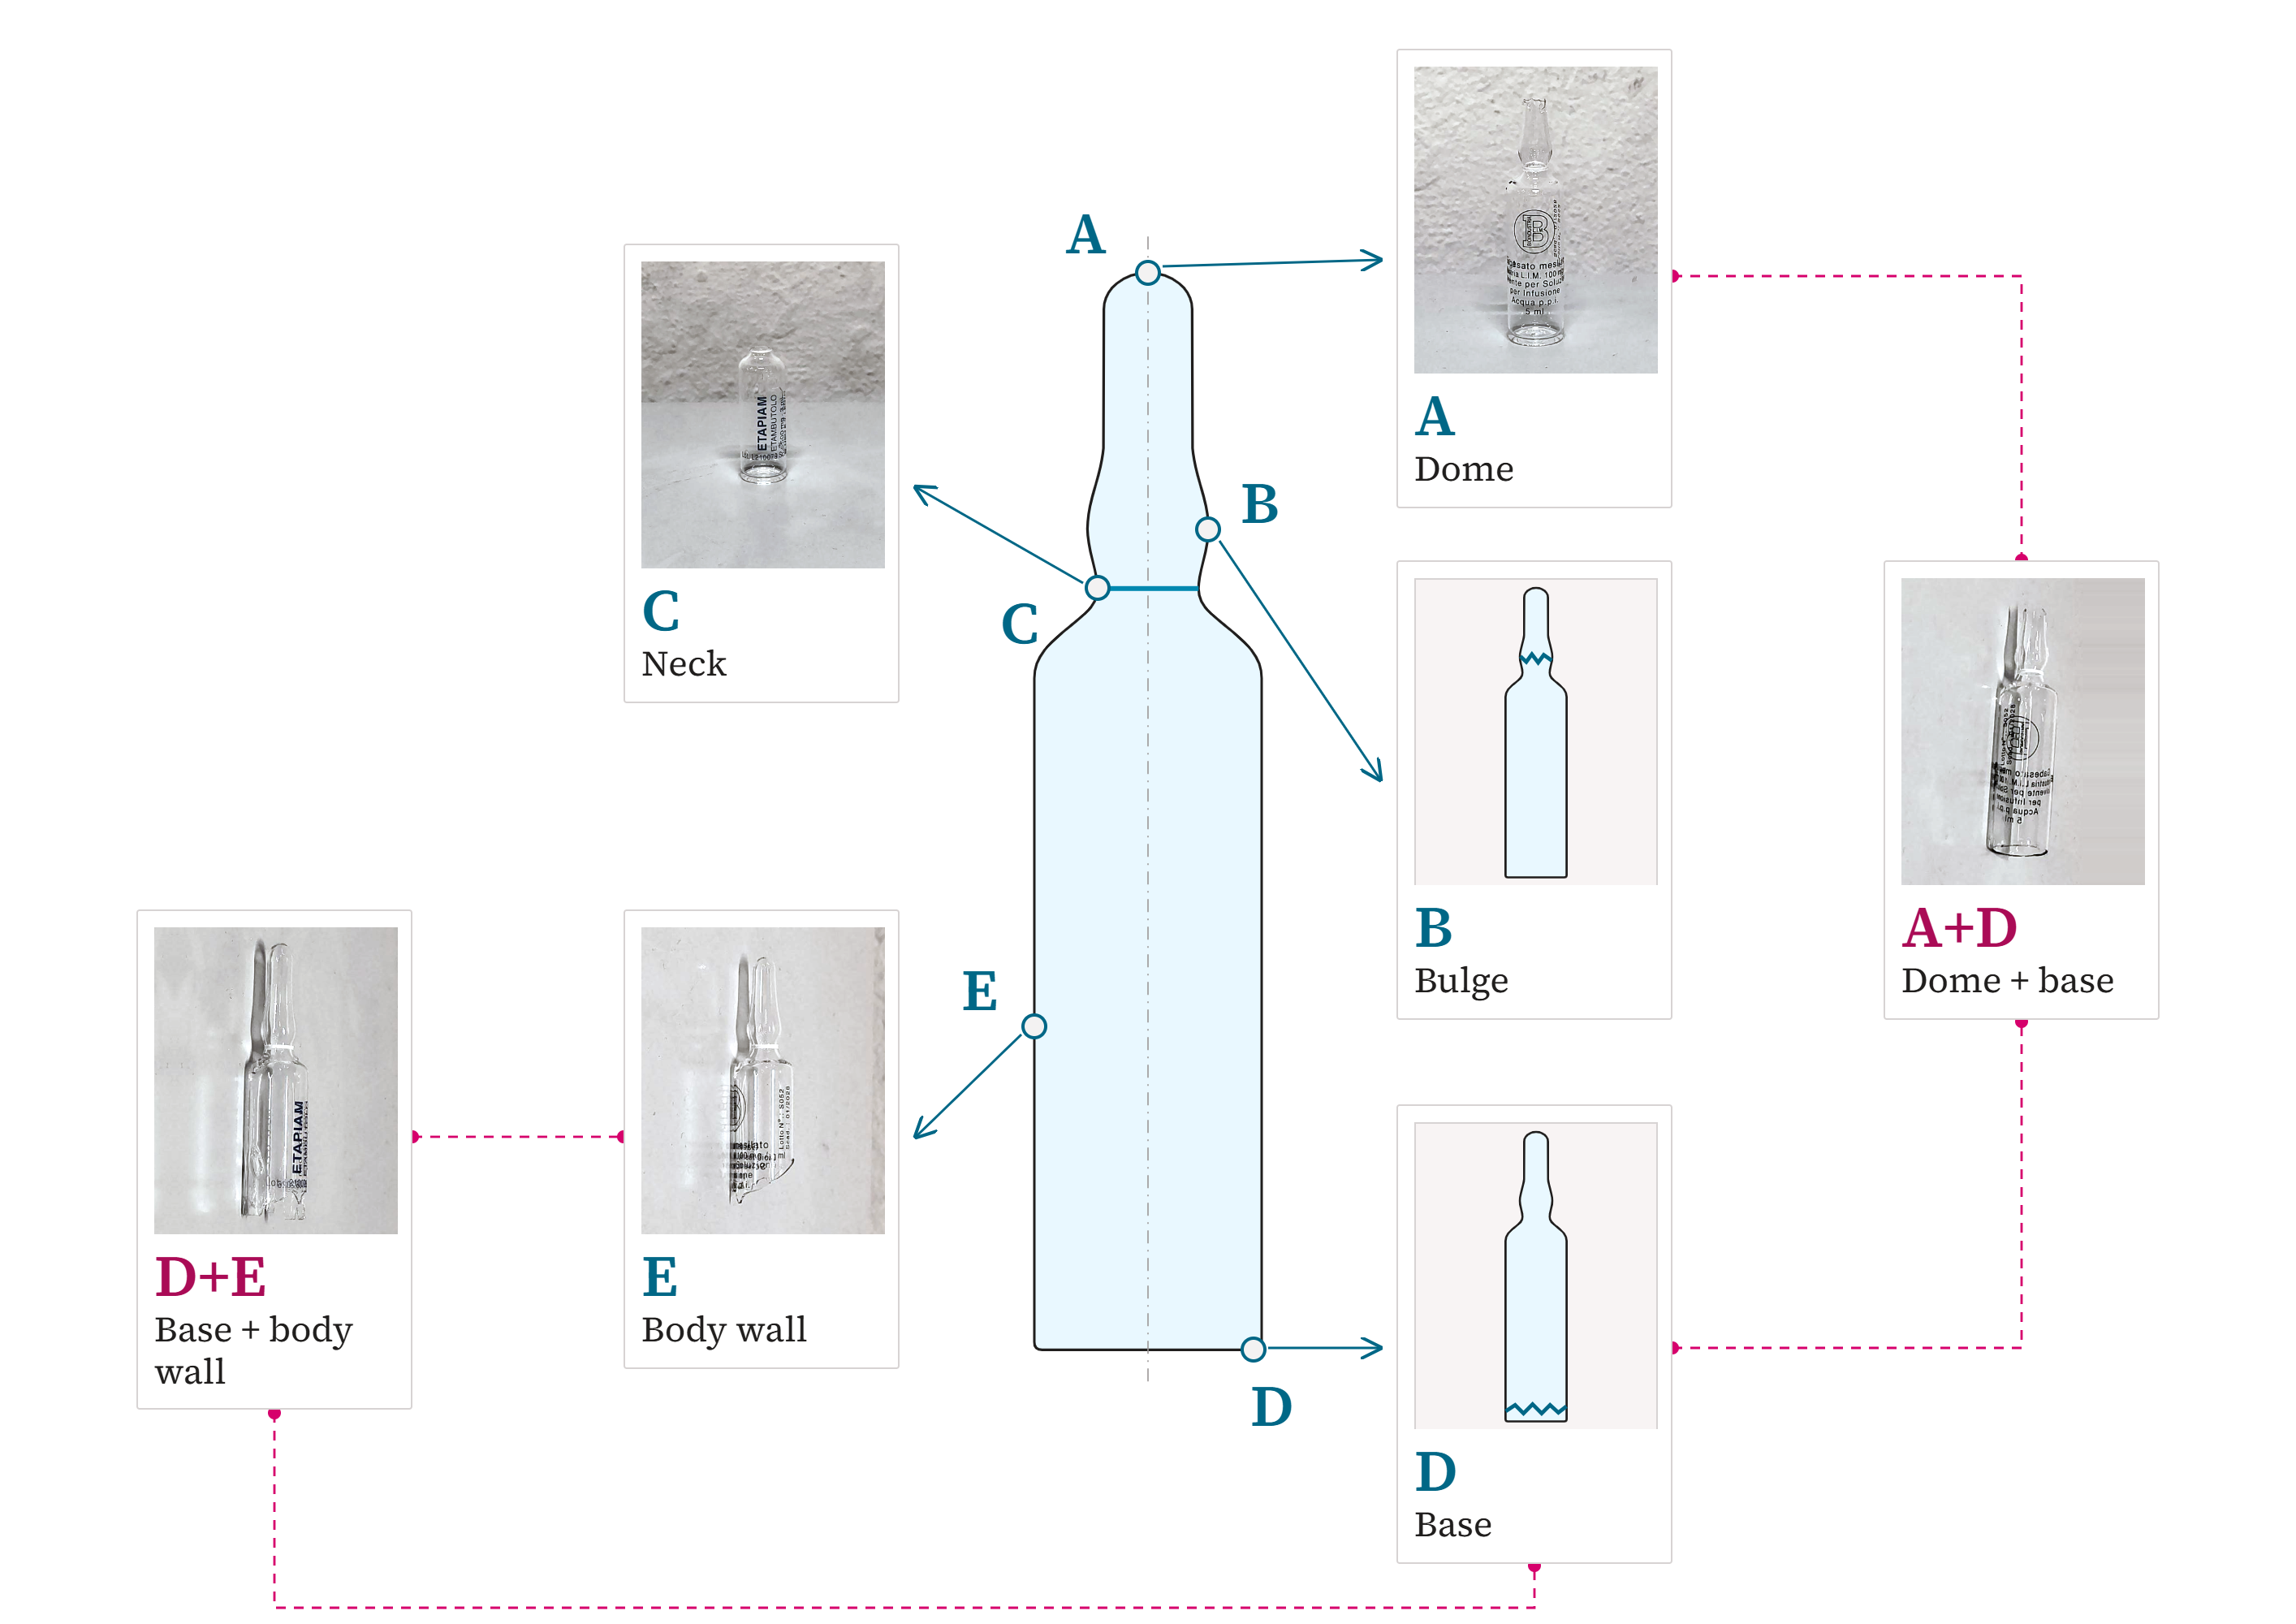
\includegraphics[width=0.9\textwidth]{figures/chap4/step1-exp/breaking_modes_schematics.png}
    \caption{Observed phial breaking modes: \textit{Dome} (A), \textit{Bulge} (B), \textit{Neck} (C), \textit{Base} (D) and \textit{Body Wall} (E), together with examples of hybrid modes (A+D and D+E).}
    \label{fig:breaking-modes}
\end{figure}

A quantitative synthesis of the data gathered experimentally about phial failure trends can be seen in \cref{fig:breaking-mode-pie}, which categorises the 76 tested phials depending on the observed failure mode. In addition to stiffness and failure load ranges observed for the individual modes, the table in \cref{fig:breaking-mode-pie} also gives some insights about the correlation between the parent medicinal batch (A or B) and the failure mechanisms. For example, the first row of the table shows that among all the 76 tested phials, 27 of them broke in mode A (dome). Within these 27 phials, 70\% belonged to Batch A, and the remaining 30\% to Batch B ("Batch mix" column). Furthermore, 53\% of all phials of Batch A broke in failure mode A, while only 20\% of Batch B showed the same failure mode ("\% of batch with this mode" column). Looking instead at the second row of the table, it is possible to see that 18 phials broke in mode E (main body), 89\% of them belonging to medicinal Batch B and representing 40\% of the entire batch. These two rows give an important insight regarding the \textit{design} of the two medicinal batches. Although nominally identical, batches A and B show different typical failure modes, where batch A favours mode A, and Batch B favours mode E. Generalising this line of reasoning, geometrically identical (as supposedly standard) phials coming from different pharmaceutical producers show radically different mechanical behaviour. 

Diverging phial behaviour can be retraced to their manufacturing processes. The phials are originally manufactured open, featuring an aperture in place of the dome to allow them to be filled with the medicinal product. At a later stage, the upper part of the glass is melted and reshaped into the dome. Depending on the medical content, varying levels of control are implemented into the thermal treatment of the phial, as the primary requirements are functionality (breaking in the designed necking when opening the phial) and transportability (complying with packaging and transportation standards \hl{CITE STANDARD HERE}), over process control. Therefore, it is entirely acceptable for different phials to exhibit distinct mechanical behaviours, even under identical loading conditions and nominally identical geometries, at the cost of needing to differentiate between pharmaceutical batches to draw any significant conclusions on material mechanics.

\begin{figure}[h!]
    \centering
    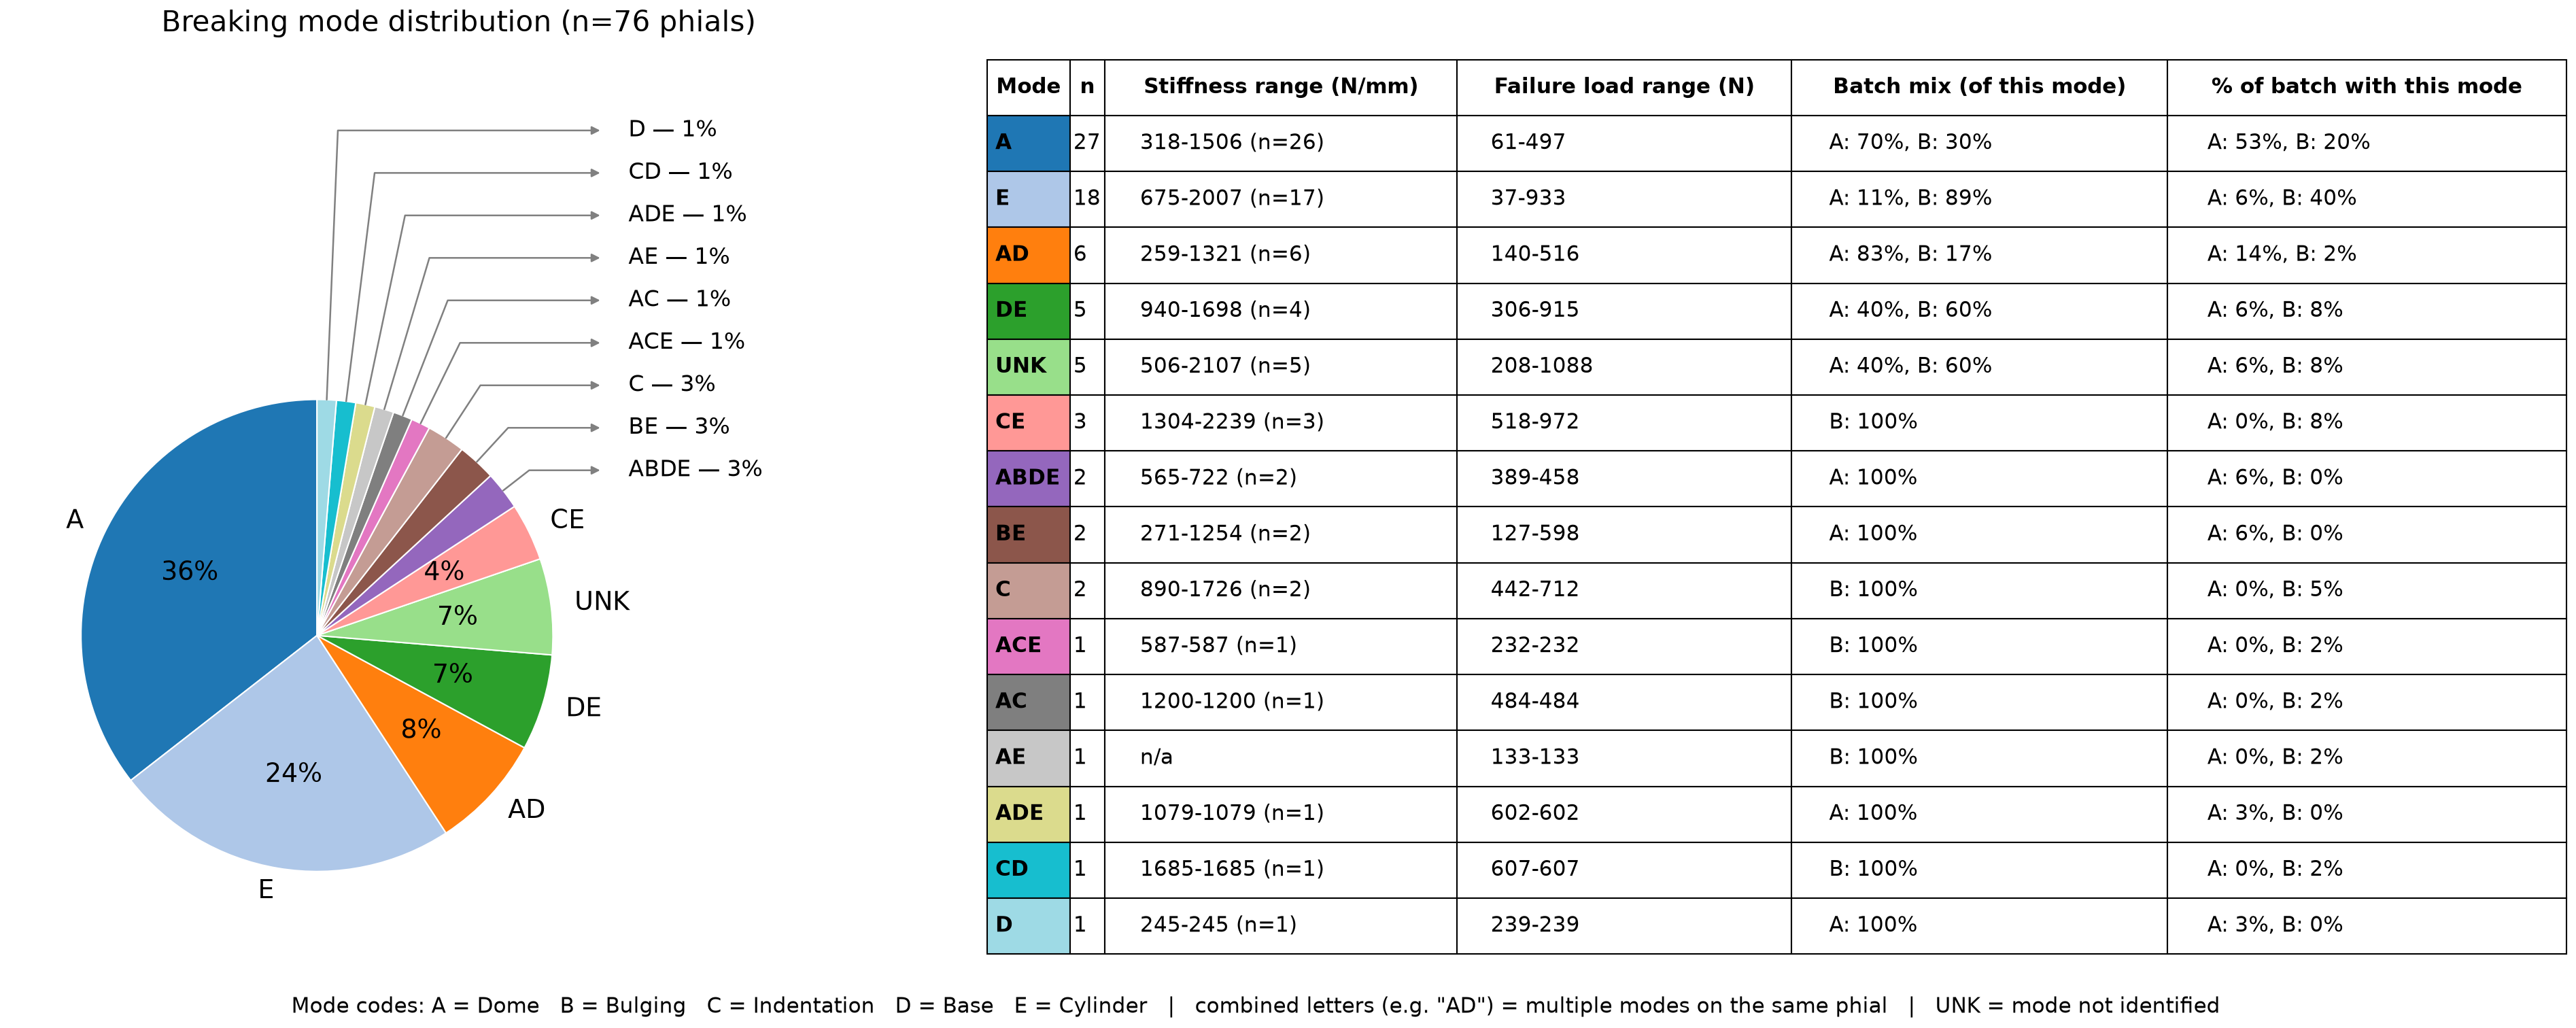
\includegraphics[width=\textwidth,height=0.45\textheight,keepaspectratio]{figures/chap4/step1-exp/breaking_mode_pie.png}
    \caption{Breaking modes observed over the 76 tested phials. Left: share of each single and hybrid mode. Right: number of phials, stiffness range and failure load range for each mode, with its split between the two batches (\textit{Batch mix}) and the fraction of each batch that failed in that mode (\textit{\% of batch with this mode}).}
    \label{fig:breaking-mode-pie}
\end{figure}


\subsubsection{Stiffness data - glass phials and PETG adaptor}
Out of the total 76 phials tested, only 65 phials were considered for the present stiffness analysis, with the remainder omitted due to unprocessability of the gathered data. Load-displacement curves were extracted from the raw dataset to construct the stiffness plot shown in \cref{fig:stiffness-overlay}. To isolate the elastic part of the structural response, data recorded after the first breaking point was discarded for each phial, as the load-bearing capacity of the phials became compromised beyond this threshold. Moreover, knowing that the primary objective of the investigation is to characterise the phials failure load to avoid medical content dispersion during a phial drop event, it is acceptable to deem post-failure behaviour irrelevant.

Categorising the results by batch reveals that Batch B exhibits a visually distinct, generally higher stiffness compared to Batch A, reinforcing the observation that different batches display significantly different mechanical behaviour. Given that thermal treatments typically do not influence stiffness, this discrepancy suggests potential diversity in geometry, disproving the assumption made in the \textit{Test article} section presented earlier. Specifically, a thicker wall in Batch B's phials would account for both higher stiffness and an increased failure load, assuming a comparable failure stress under the current compressive loading state.

Across all curves, an initial compliant branch is observed. This could be attributable to experimental setup constraints as the phials settle and slide into proper contact before effective load transfer occurs. The response remains predominantly elastic across the observed stiffness range, with minor softening observed around 800\,N, which is associated with the stiffness compliance of the PETG adaptor (a similar "step" is observed in \cref{fig:petg-stiffness} at comparable loads, indicating some sort of elastic instability in the response of the adaptor). Moreover, a degree of random error must be considered regarding perfect alignment within the PETG adaptor. Deviations from perfect verticality (caused either by clearance between the adaptor and the phial or by subtle manufacturing phial shape imperfections) have a significant influence on the measured stiffness. This aspect is further investigated in the FEM model presented in \cref{section:step2-fem-compression}, which proposes considerations on initial geometric defects to evaluate their impact on overall phial stiffness.


\begin{figure}[h]
    \centering
    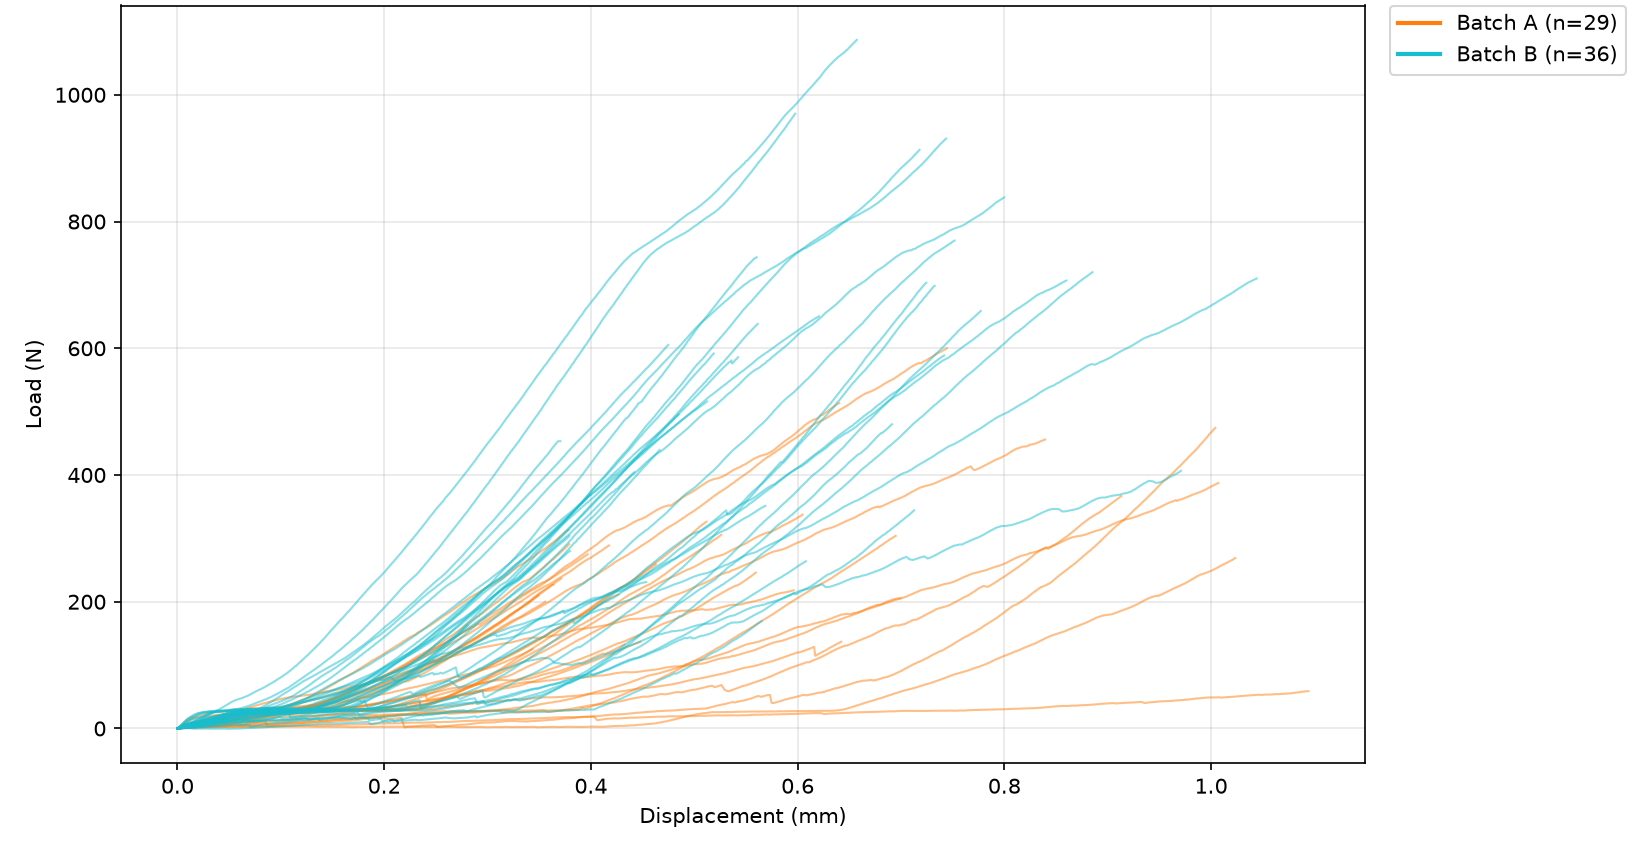
\includegraphics[width=\textwidth]{figures/chap4/step1-exp/stiffness_overlay_experimental_only.png}
    \caption{Experimental load-displacement curves of all tested phials up to the failure point, grouped by batch (Batch A, $n=29$; Batch B, $n=36$).}
    \label{fig:stiffness-overlay}
\end{figure}


In retrospective of completing the present experimental campaign and its FEM modelling in \cref{section:step2-fem-compression}, further attention had to be given to the strong limitations of the experimental setup. To validate the stiffness data gathered, it was necessary to conduct a separate investigation on the mechanical compliance of the setup, to determine experimentally the stiffness of the PETG adaptor. For this scope, the adaptor was subjected to the same loading configuration used for the glass phials (refer to \cref{fig:compression_setup} for clarification), using a 15cm steel bar of comparable diameter to the glass phials (considered infinitely rigid compared to the PETG structure) to compress the component directly without the risk of inducing instabilities or buckling. The PETG adaptor's load-displacement data is shown in \cref{fig:petg-stiffness}, which evaluates the adaptor stiffness at a nominal value of 2037\,N/mm obtained by a linear fit within the load band of Mode a failures. Furthermore, it is possible to notice that slight softening behaviour occurred at approximately 800\,N, introducing a step-like feature that matches the response observed in the high-load regime of the glass phial tests. 

\begin{figure}[htbp]
    \centering
    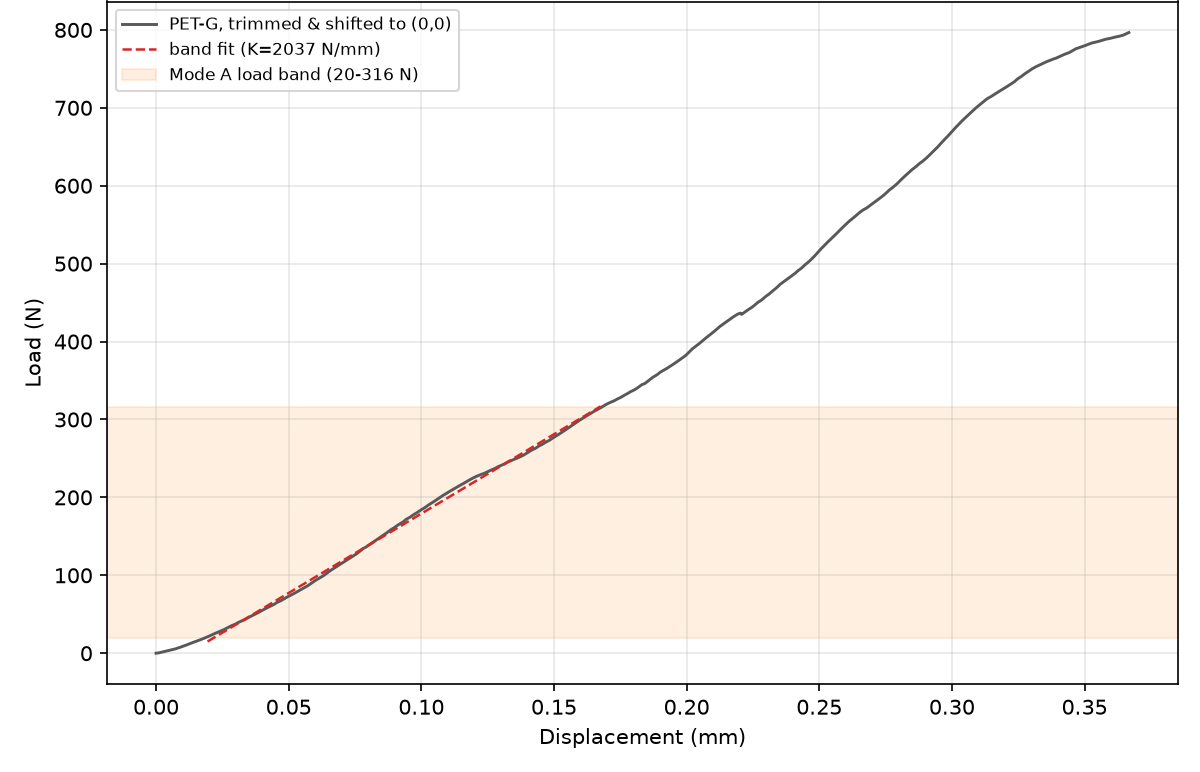
\includegraphics[width=0.85\textwidth]{figures/chap4/step1-exp/petg_raw_curve_analysis.png}
    \caption{Load-displacement curve of the PETG adaptor, trimmed and shifted to the origin. The adaptor stiffness, $K_{PETG} = 2037$\,N/mm, is obtained by a linear fit within the load band of Mode A failures (20-316\,N).}
    \label{fig:petg-stiffness}
\end{figure}

Overall, PETG adaptor stiffness serves as a critical datum for reconciling experimental stiffness with numerical predictions of the FEM model presented later. Notably, calculating the adaptor stiffness was not originally planned during the test campaign, but rather it was performed post-hoc to resolve a significant mismatch observed between the empirical stiffness measurements and the initial numerical predictions.


\subsubsection{Failure load extraction}
\Cref{fig:weibull-combined} displays the brittle failure points extracted from the experimental load-displacement curves for all 76 tested phials, categorised by batch and fitted to a two-parameter Weibull distribution. The top plot illustrates the fitted two-parameter Weibull probability density functions, highlighting the 1st and 5th percentiles of each curve, while the bottom plot details the individual failure loads grouped by batch and displacement rate. An analysis of these Weibull distribution plots indicates that while clear stiffness data could not be extracted for every sample, a definitive failure load was successfully obtained across the entire dataset of 76 phials. These failure loads were plotted collectively, regardless of the observed failure mode, to provide an objective picture of the failure loads independent of the manual, visual classification of individual failure modes.

\begin{figure}[htbp]
    \centering
    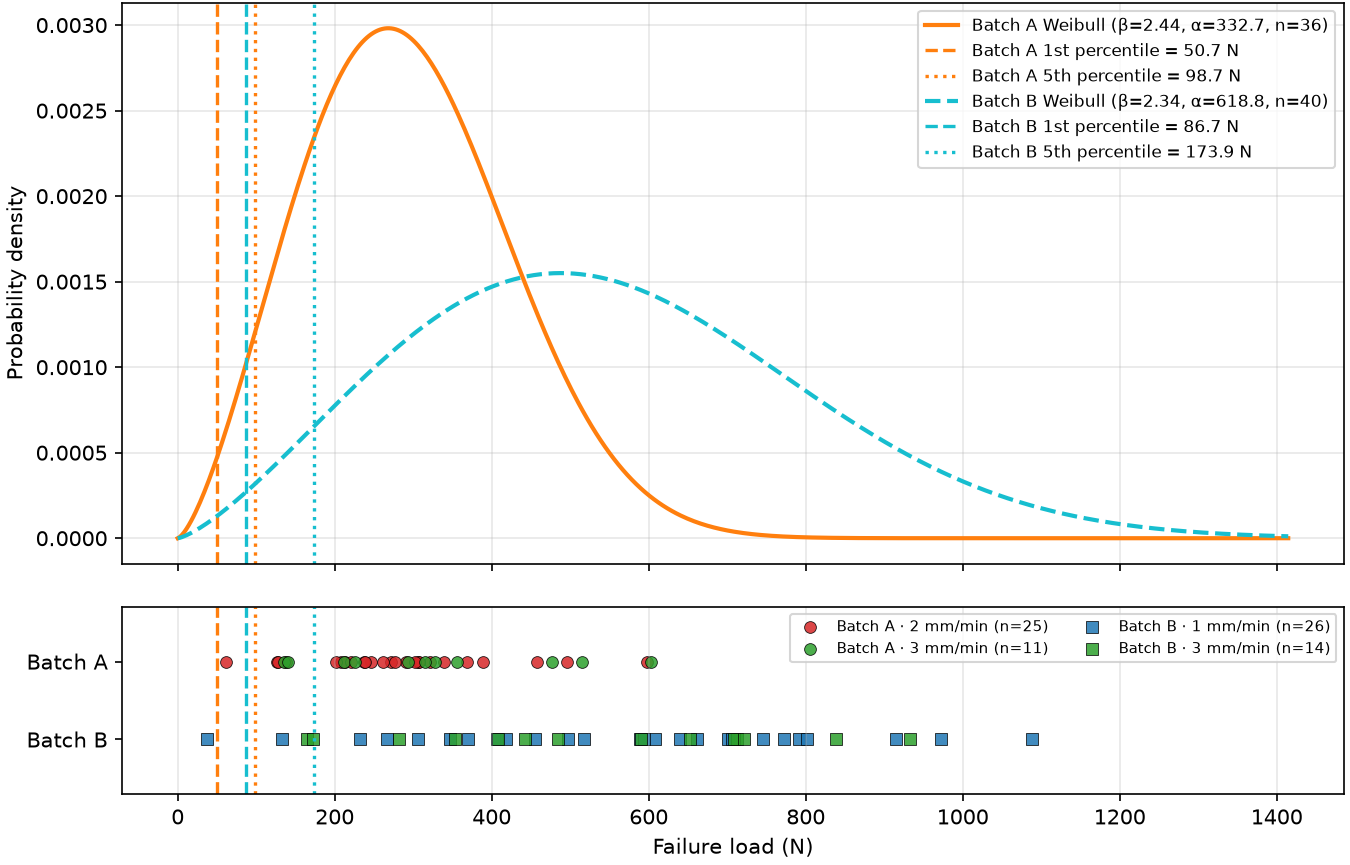
\includegraphics[width=0.85\textwidth]{figures/chap4/step1-exp/weibull_combined.png}
    \caption{Failure load distributions of Batch A and Batch B. Top: fitted two-parameter Weibull probability density functions, with the 1st and 5th percentiles marked. Bottom: individual failure loads, grouped by batch and displacement rate.}
    \label{fig:weibull-combined}
\end{figure}

The resulting Weibull distribution highlights that Batch A exhibits a lower characteristic failure load but lower scatter, whereas Batch B shows a higher mean failure load alongside higher dispersion. Consequently, Batch A offers greater reliability for statistical and mechanical analysis and is therefore the only batch considered for the analysis from this point forward. Furthermore, these plots confirm that the testing rate had a negligible effect on the results, as evidenced by the lack of correlation between experimental outcomes and load application speed.



\subsubsection{Step 1 deliverable: design failure load of the phial}
Based on the considerations made previously, the summary dataset presented in \cref{tab:step1-summary-data} is selected as the baseline datum to feed into the subsequent stage of the airbag design workflow.

\begin{table}[h!]
\centering
\caption{Experimental data selected for the calibration of the FEM glass material.}
\label{tab:step1-summary-data}
\begin{thesistable}{
  colspec = {X[1.3,l] X[1,l] X[1.6,l]},
}
Quantity & Value & Source / note \\
Target failure load ($F_{fail}$) & \qty{98.7}{\newton} & Batch A, Weibull 5th percentile ($\beta=2.44$, $\alpha=\qty{332.7}{\newton}$, $n=36$) \\
Mode A stiffness & 318\,N/mm - 1506\,N/mm & Dome failure; \qty{53}{\percent} of Batch A \\
Mode AD stiffness & 259\,N/mm - 1321\,N/mm & Dome + base failure; \qty{14}{\percent} of Batch A \\
PETG adaptor stiffness & 2037\,N/mm & Linear fit, 20\,N-316\,N band (\cref{fig:petg-stiffness}) \\
\end{thesistable}
\end{table}



\FloatBarrier % keep the Step 1 figures and table inside Section 4.2
